\documentclass{article}
\usepackage[pdftex]{graphicx}

\title{Estimating and Handling Uncertainties in the Laboratory}
\author{John P. Cummings}
\date{Fall 2020}

\begin{document}
\maketitle

\section{Introduction}
The estimation of uncertainties is somewhat of an artform rather than a science.  Many assumptions are often made to give some rigor to this art; unfortunately we often forget the assumption when applying the procedures derived.  Don't forget to use your common sense.

Please {\em don't} use percent deviation.  
\begin{equation}
\% {\rm deviation} ~=~ {{ \rm measured} - {\rm accepted } \over {\rm accepted }} \times 100
\end{equation}
Although this can be interesting in rare cases, it is almost never used appropriately.  The much more interesting value is the uncertainty of the measured value: in other words, if we repeated the measurement how different is it likely to be? 

\section{Uncertainties}

\subsection{Device Resolution}
One common source of uncertainty in the lab is due to the resolution of the measuring device used.  For example a scale will have a smallest division, whether it is a ruler, an analog electrical meter, a clock scale, {\em etc.}  For a reasonably graduated scale the uncertainty is usually about equal to the smallest division.  Imagine the possible readings a reasonable person might make for a given measurement.  Vernier scales require a little more thought, the resolution might depend on the quality and width of the division marks.

If the device is digital, it will often have a specified resolution.  The trick can be to locate it.  Sometimes it will be on a plate or sticker on the device itself.  Check the back or bottom of the instrument if it is not apparent.  You might have to refer to the manual which may be in the lab.  If you cannot find the manual in the lab, you may be able to locate it online.  In the absence of any manufacturer specification, you probably will be close if you use $1/2$ the last digit (and common sense).

\subsection{Random or Statistical}
Some measurements will be dominated by other random contributions.  Take for example measuring the period of a pendulum with a stopwatch.  Repeated measurements will lead to slightly different results due to your reaction time, {\em etc.}  Here we make some assumptions referred to earlier, such as the distribution of results is random and normal (or Gaussian).  In other words, if we repeated the measurement many time and produced a {\em histogram} of the results we assume we would get a Gaussian distribution.

\begin{figure}
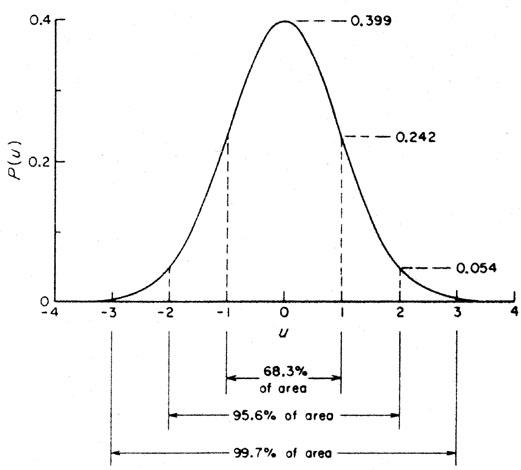
\includegraphics[width=4in]{images/gaussian.jpg}
\caption{A gaussian distribution.}
\label{fig:gaussian}
\end{figure}

Under these assumptions, statisticians have shown that the best estimate of the true value is given by the mean $\mu$ which we all know is

\begin{equation}
\mu = { 1 \over N } \sum_i^N x_i
\end{equation}

where $x_i$ are the sum is over all $N$ measurements.  Great, this gives us the best guess of the value, but what about it's uncertainty?  The {\em width} of the distribution of results is indicative of its uncertainty.  We can measure the width by looking at the average deviation of the results from the mean.  Notice that the signed deviation of a symmetric distribution from the mean is always zero (not very useful) so we must somehow get rid of the sign.  We take the square of the difference $x_i - \mu$ and average
\begin{equation}
\sigma^2 = {1\over N} \sum_i^N \left( x_i - \mu \right)^2
\end{equation}
Sometimes you'll see the $N$ replaced with $N-1$ to give you something called ``an unbiased estimator.''  Either is fine for this class, and the difference for large $N$ is negligible anyway.

This technique of repeated measurements is useful if the other techniques above don't apply.  You could also use it to {\em measure} the resolution of a device or measurement technique for use during future measurements.

\subsection{Systematic}

Systematic uncertainties are much harder to quantify in a general fashion.  Since they can systematically move the measurement away from the correct value, averaging will not neccessarily remove these no matter how many measurements you make.  This property can often serve as a useful test to classify an uncertainty as statistical or systematic: would repeated measurements tend to decrease the size of the uncertainty?  Systematic uncertainties can come from the measurement devices used or from assumptions and approximation used in the analysis of your data.  Typical sources in this lab might be things like an uncalibrated instrument, or the assumption that a wire is zero resistance.

\section{Propagation of Errors}

When measured values are used to calculate quantities it is important to propagate the error on the measured quantity through to the calculated value.  For a simple function of one measured variable it is easy to see (Figure~\ref{fig:error-prop})
\begin{figure}
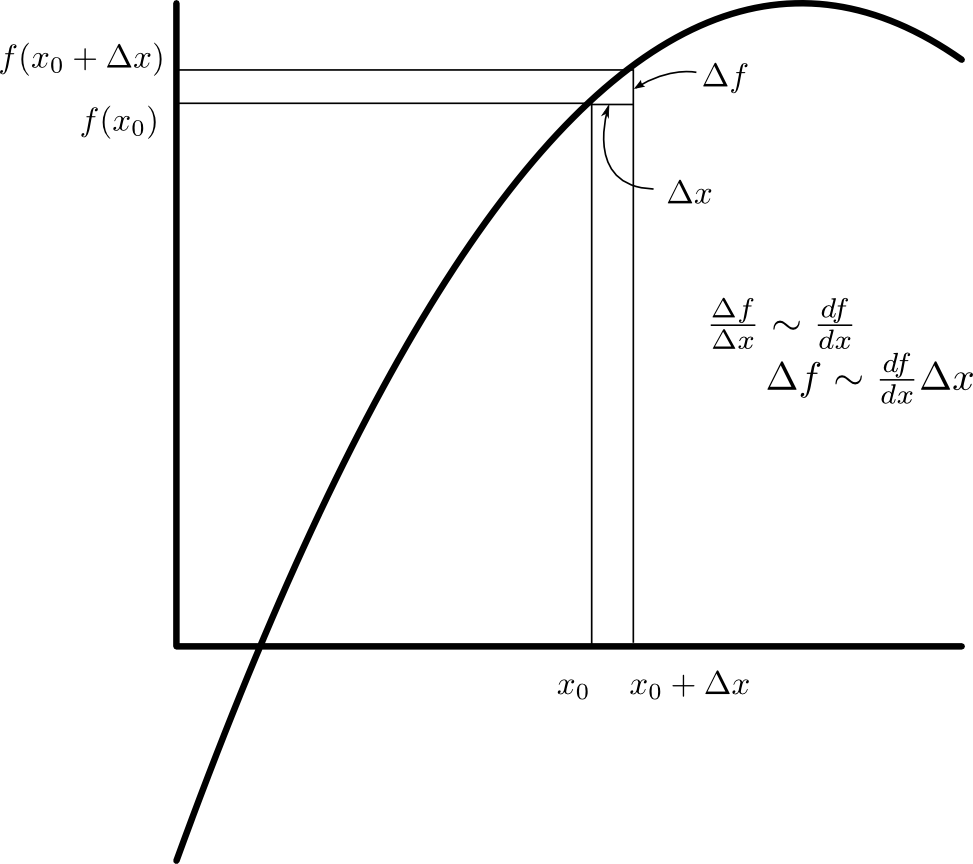
\includegraphics[width=3in]{images/error-prop.png}
\caption{Propagating error}
\label{fig:error-prop}
\end{figure}
that the trick is to multiply the measured error by the derivative of the function with respect to the measured variable:
\begin{equation}
\sigma_f = {df \over dx} \sigma_x
\end{equation}

When the calculated value is a function of more than one measured quantities, the total error is found by adding the individual errors in quadrature (or adding the squares of the errors)
\begin{equation}
\sigma_f^2 = \sum_i ({df \over dx} \sigma_i)^2
\label{eq:error-prop}
\end{equation}

For example, suppose you have measured the mass $m$ of an object and it's acceleration $a$ and you wish to calculate the force $F$ from Newtons law
\begin{equation}
F = ma.
\label{eq:newton}
\end{equation}
You measured the mass to be $m = 550.10~ {\rm g}$ and the scale has a resolution of $\sigma_m = 0.02 ~{\rm g}$.  The acceleration you measured was $a = 43 ~{\rm cm}/{\rm s}^2$ and the accelerometer has a resolution of $\sigma_a = 5 ~{\rm cm}/{\rm s}^2$.  You would record these values as $m = 550.10 \pm 0.02 ~{\rm g}$ and $a = 43 \pm 5 ~{\rm cm}/{\rm s}^2$.

To calculate the central value of $F$, simply us the central value for the measured quantities in Eq.~\ref{eq:newton}:
\begin{equation}
F = 550.10 ~{\rm g} \times 43~ {\rm cm}/{\rm s}^2 = 23654 ~{\rm dynes}
\end{equation}

To calculate the uncertainty, use Eq.~\ref{eq:error-prop}.
\begin{eqnarray*}
\sigma_F^2 &=& \left( {dF \over dm} \sigma_m \right)^2 + \left( {dF \over da} \sigma_a \right)^2 \\
&=& \left( a \sigma_m \right)^2 + \left( m \sigma_a \right)^2 \\
&=& \left( 43 ~{\rm cm}/{\rm s}^2\times  0.02 ~{\rm g} \right)^2 + \left( 550.1 ~{\rm g}\times  5~ {\rm cm}/{\rm s}^2\right)^2 \\
&=& 7.56\times 10^6 ~{\rm dynes^2}
\end{eqnarray*}
so $\sigma_F = 2750 ~{\rm dynes}$, and your final answer should be written
\begin{equation}
F = 24000 \pm 3000 ~{\rm dynes}.
\end{equation}
where we have rounded the uncertainty to one significant figure--if we are already uncertain in the thousands place, it is silly to be reporting hundreds and smaller places!  The central value should then be written no more accurately that this number.  The general rule is round the error to one (or sometimes two, for an intermediate result) significant digits and then use that as the lowest decimal place of the quoted value.  

\subsection{Common cases}
There are several common cases you may wish to remember to save yourself some time:
\begin{enumerate}
\item scalar multiplication, $f(x) = cx$
\[
\sigma_f = c\sigma_x
\]
\item addition, $f(x,y) = x + y$
\[
\sigma_f^2 = \sigma_x^2 + \sigma_y^2
\]
\item a product, $f(x,y) = xy$, or division, $f(x,y) = x/y$
\[
\left( \frac{\sigma_f}{\bar{f}} \right)^2 = \left( \frac{\sigma_x}{\bar{x}} \right)^2 + \left( \frac{\sigma_y}{\bar{y}} \right)^2
\]
(combine the {\em fractional uncertainties} as you would for addition.)
\end{enumerate}


\section{Significant Digits}

If you have no knowledge of the resolution (for example, in a practice problem from a book) pay attention to significant digits!  Please don't write down every digit your calculator gives you (unless it is justified).  Ignoring this rule can lead to false conclusions.  Consider the case of Olympic gymnastics: judges give scores to the tenth of a point and the scores are averaged.  Yet medals are given out based on results to the thousandths place.  Can you come up with a scenario where the wrong medals are given out?

The number of significant digits is usually the digits in a number after dropping any leading zeros.  This is not always unambiguous, for instance trailing zeros when there is no decimal point as in 310 can be troublesome.  Again, use common sense and be careful when you record values.  A nice convention is to write the values of physical measurements so that the last measured digit falls to the right of the decimal point.  You can do this by either using scientific notation or simply choosing a larger unit of measurement.

With most arithmetic operations you should keep in your answer the {\em fewest} number of significant digits you have in your data.  The only exception is when adding (or subtracting) numbers when you use the fewest number of {\em decimal places} in your data.  Consider $103.25 - 0.0001$

\section{Exercises}

\begin{enumerate}
\item Measure the width and length of the whiteboard, and calculate the error.
\item Measure and calculate the density of some metal shapes.  Compare your answer with others in the class and try to identify which are made of the same material.


\end{enumerate}

\end{document}
